%%This is a very basic article template.
%%There is just one section and two subsections.
\documentclass[english,a4paper]{report}

\usepackage{graphicx}
\usepackage{listings}
\usepackage{color}
\usepackage{makeidx}
\usepackage{hyperref}
\usepackage{parskip}

\usepackage{tikz}
\usetikzlibrary{shapes,arrows}

\usepackage{multirow}
\usepackage{tocloft}
\renewcommand{\cftsecaftersnumb}{\hspace{6em}}
\renewcommand{\cftsubsecaftersnumb}{\hspace{6em}}
\renewcommand{\cftsubsubsecaftersnumb}{\hspace{6em}}

\makeindex

\hypersetup{
    %bookmarks=true,         % show bookmarks bar?
    unicode=false,          % non-Latin characters in Acrobats bookmarks
    pdftoolbar=true,        % show Acrobats toolbar?
    pdfmenubar=true,        % show Acrobats menu?
    pdffitwindow=false,     % window fit to page when opened
    pdfstartview={FitH},    % fits the width of the page to the window
    pdftitle={TFE4140 - Assignment 1 - hvatum},    % title
    pdfauthor={Stian Hvatum},     % author
    pdfsubject={TFE4140 Modeling and Analysis of Digital Systems},   % subject of the document
    pdfcreator={Stian Hvatum},   % creator of the document
    pdfproducer={Stian Hvatum}, % producer of the document
    pdfnewwindow=true,      % links in new window
    colorlinks,       % false: boxed links; true: colored links
    linkcolor=black,          % color of internal links
    citecolor=green,        % color of links to bibliography
    filecolor=magenta,      % color of file links
    urlcolor=cyan           % color of external links
}

\definecolor{listinggray}{gray}{0.9}
\definecolor{lbcolor}{rgb}{0.9,0.9,0.9}

\renewcommand{\thesection}{Task \arabic{section}}
\renewcommand{\thesubsection}{\arabic{subsection}}
\renewcommand{\thesubsubsection}{\arabic{subsubsection}.}

\title{TFE4140 Modeling and Analysis of Digital Systems\\
\Huge Assignment 1}
\author{Stian Hvatum (hvatum)\\MTDT}

\begin{document}
\maketitle
%\tableofcontents
\newpage
\section{}
\subsection{}
(reading done)
\subsection{}
\begin{figure}
% Define block styles
\tikzstyle{decision} = [diamond, draw, fill=blue!20, 
    text width=4.5em, text badly centered, node distance=3cm, inner sep=0pt]
\tikzstyle{block} = [rectangle, draw, fill=blue!20, 
    text width=5em, text centered, rounded corners, minimum height=4em]
\tikzstyle{line} = [draw, -latex']
\tikzstyle{cloud} = [draw, ellipse,fill=red!20, node distance=3cm,
    minimum height=2em]
    
\begin{tikzpicture}[node distance = 2cm, auto]
    % Place nodes
    \node [block] (start) {Fetch first statement};
    \node [cloud, left of=start] (load) {Load VHDL};
    \node [block, below of=start] (eval) {Evaluate statement};
    \node [decision, below of=eval] (changed) {Left side changed?};
    \node [block, anchor=center] (add) at (-3, -7) {Add new statements to event queue at NOW + delay};
    \node [decision, below of=changed, node distance=4cm] (more) {More statements in event queue};
    \node [block, below of=more, node distance=4cm] (end) {Simulation done};
    \node [block, right of=changed, node distance=3cm] (next) {Fetch next statement};
    % Draw edges
    \path [line] (start) -- (eval);
    \path [line] (eval) -- (changed);
    \path [line] (next) |- (eval);
    \path [line] (add) |- (more);
    \path [line] (changed) -| node [near start] {yes} (add);
    \path [line] (changed) -- node {no}(more);
    \path [line] (more) --  node{no}(end);
    \path [line] (more) -| node [near start]{yes}(next);
    \path [line,dashed] (load) -- (start);
\end{tikzpicture}

\caption{Simulation Cycle}
\label{dia:simcycle}
\end{figure}
As we see in figure \ref{dia:simcycle}, a VHDL simulation cycle begins with fetching the first statement.
The first statement is the topmost line in the topmost process.
When we evaluate the statement, if the left side, $Y$, of the statement changes its value, then we have to add
all statements that depends on $Y$ to a dynamic event queue. This new event is added at current time + some given delay.

As the event queue is sorted by event time, all events will be processed in order. When the system comes to a state where no more
events occur, and the queue of events are empty, the simulation has come to an end.

\subsection{}
When no delay is explicitly specified for a statement, it implies a delay of zero. Since this might introduce changes to the
event queue in such a way that statement order matters, we add a so called \textit{delta delay} to the time which event is queued for.
The delta delay is an infinitesimal amount of time, such that the changes are reflected before the next real time step,
and do not interfere the already queued events.

\section{}
\subsection{}
\begin{tabular}{l|c|c|c|c|c|c|l}
%    \hline
    Time	&A	&B	&Q	&QN	&Q+	&QN+	&Activated processes\\
    \hline
    \hline
    %%%%%%%%%%%%%%%%%%%%%%%%%%%%%%%%%%%%%%%%%%%%%%%%%%%%%%%%%%%%%%%%%%%%%%
%%                                                                  %%
%%  This is a LaTeX2e table fragment exported from Gnumeric.        %%
%%                                                                  %%
%%%%%%%%%%%%%%%%%%%%%%%%%%%%%%%%%%%%%%%%%%%%%%%%%%%%%%%%%%%%%%%%%%%%%%
$0$	        &U	&U	&U	&U	&	&	&Initializing, A,B activated\\
$0+\Delta$	&1	&0	&	&	&0	&X	&Q,QN\\
$0+2\Delta$	&	&	&0	&X	&(0)	&1	&Q,QN\\
$0+3\Delta$	&	&	&(0)	&1	&	&(1)	&Q\\
$0+4\Delta$	&	&	&	&(1)	&	&	&No change, suspend\\
\hline
    \hline
$10$	        &	&	&	&	&	&	&A activated\\
$10+\Delta$	&0	&	&	&	&(0)	&	&Q\\
$10+2\Delta$	&	&	&(0)	&	&	&	&No change, suspend\\
\hline
    \hline
$20$	        &	&	&	&	&	&	&B activated\\
$20+\Delta$	&	&1	&	&	&	&0	&QN\\
$20+2\Delta$	&	&	&	&0	&1	&	&Q\\
$20+3\Delta$	&	&	&1	&	&	&(0)	&QN\\
$20+4\Delta$	&	&	&	&(0)	&	&	&No change, suspend\\
\hline
    \hline
$30$	        &	&	&	&	&	&	&B activated\\
$30+\Delta$	&	&0	&	&	&	&(0)	&QN\\
$30+2\Delta$	&	&	&	&(0)	&	&	&No change, suspend\\
\hline
    \hline
$40$	        &	&	&	&	&	&	&A,B activated\\
$40+\Delta$	&1	&1	&	&	&0	&(0)	&Q,QN\\
$40+2\Delta$	&	&	&0	&(0)	&	&(0)	&QN\\
$40+3\Delta$	&	&	&	&(0)	&	&	&No change, done\\
    \hline
    \hline

%    \hline
\end{tabular}
\subsection{}
The simulation stops after all stimuli has been applied.

\newpage
\subsection{}
\subsubsection{Implementation}
\lstinputlisting[language=VHDL]{../vhdl/a1.vhdl}
\newpage
\subsubsection{Testbench}
\lstinputlisting[language=VHDL]{../vhdl/test_ab_latch.vhd}
\newpage
\subsection*{Simulation}
I ran my testbench in ISim. The results can be seen in figure \ref{img:isim}

\begin{figure}[h!]
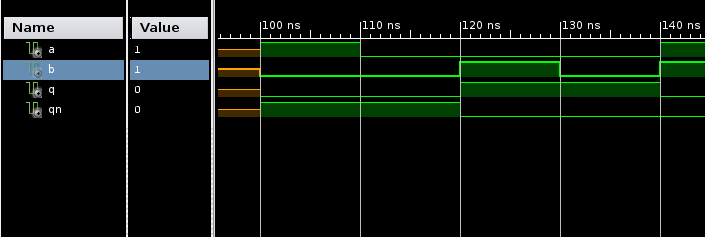
\includegraphics[width=14cm]{simulation.png}
\label{img:isim}
\caption{Simulating in ISim}
\end{figure}
\end{document}
